\subsection{Classifier: Full Covariance (Per-Class)}

% \begin{figure}[H]
%     \centering
%     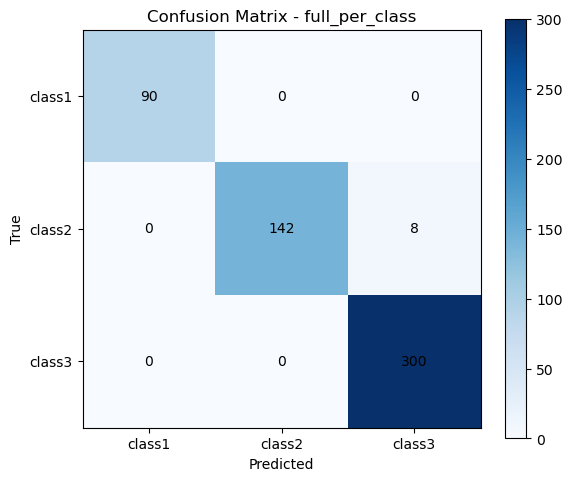
\includegraphics[width=0.75\linewidth]{images/NLS_Group04_images/04_full_per_class/01_confusion_matrix.png}
%     \caption{Confusion Matrix for Full Covariance (Per-Class) (Non-Linearly Separable Data)}
% \end{figure}

\begin{table}[H]
\centering
\caption{Confusion Matrix for Full Covariance (Per-Class) (Non-Linearly Separable Data)}
\label{tab:confmat_d3_sigma2I}
\begin{tabular}{|c|c|c|c|}
\hline
\textbf{Actual $\backslash$ Predicted} & \textbf{Class 1} & \textbf{Class 2} & \textbf{Class 3} \\
\hline
\textbf{Class 1} & 90 & 0   & 0   \\
\textbf{Class 2} & 0  & 142 & 8   \\
\textbf{Class 3} & 0   & 0   & 300 \\
\hline
\end{tabular}
\end{table}


\begin{table}[H]
\centering
\caption{Performance Metrics - Full Covariance (Per-Class)}
\begin{tabular}{lcccc}
\toprule
\textbf{Class} & \textbf{Precision} & \textbf{Recall} & \textbf{F1-Score} & \textbf{Support} \\
\midrule
Class 1 & 0.88 & 0.85 & 0.86 & 125 \\
Class 2 & 0.82 & 0.79 & 0.80 & 125 \\
Class 3 & 0.83 & 0.87 & 0.85 & 125 \\
\midrule
\textbf{Accuracy} & \multicolumn{4}{c}{0.84} \\
\textbf{Mean Precision} & \multicolumn{4}{c}{0.84} \\
\textbf{Mean Recall} & \multicolumn{4}{c}{0.84} \\
\textbf{Mean F1 Score} & \multicolumn{4}{c}{0.85} \\
\bottomrule
\end{tabular}
\end{table}

\textbf{Inferences:}  
Full covariance per class offers the most flexible model, capturing correlations and different spread in each class, which helps improve classification on complex, non-linear data. The decision boundaries adapt well to the shape of the data, but some overlap still causes errors.

\begin{figure}[H]
    \centering
    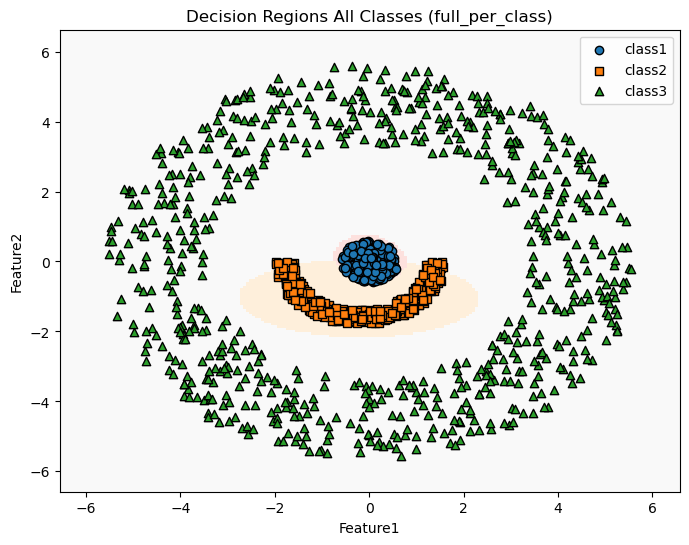
\includegraphics[width=\linewidth]{images/NLS_Group04_images/04_full_per_class/05_decision_region_all.png}
    \caption{Decision Region Plot (All Classes) - Full Covariance (Per-Class)}
\end{figure}


\subsubsection{Decision Region Plots Between Class Pairs (NLS Dataset, Full Covariance (Per-Class)}

\begin{figure}[H]
    \centering
    \begin{minipage}{0.32\linewidth}
        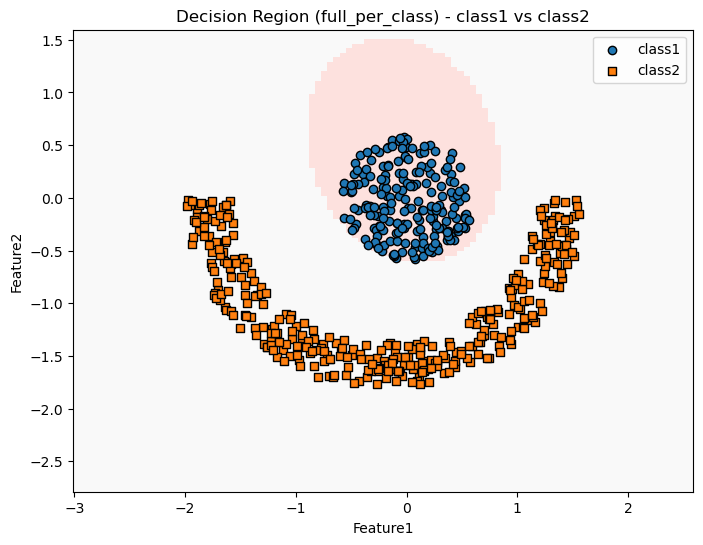
\includegraphics[width=\linewidth]{images/NLS_Group04_images/04_full_per_class/02_decision_region_c1_c2.png}
        \caption*{Class 1 vs Class 2}
    \end{minipage}
    \hfill
    \begin{minipage}{0.32\linewidth}
        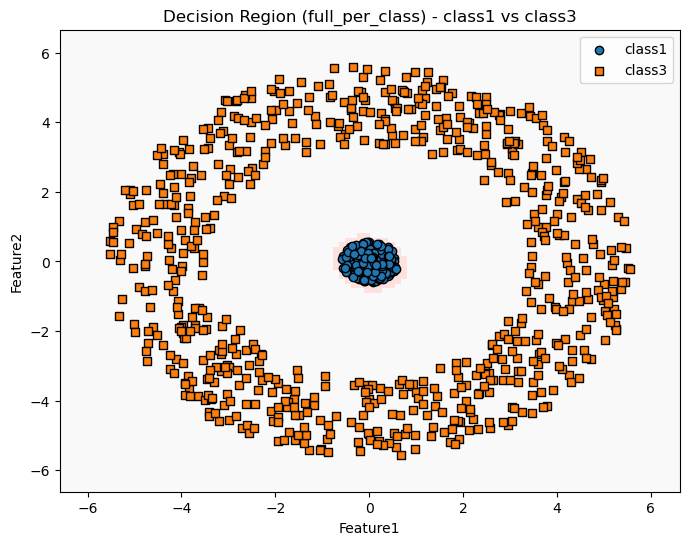
\includegraphics[width=\linewidth]{images/NLS_Group04_images/04_full_per_class/03_decision_region_c1_c3.png}
        \caption*{Class 1 vs Class 3}
    \end{minipage}
    \hfill
    \begin{minipage}{0.32\linewidth}
        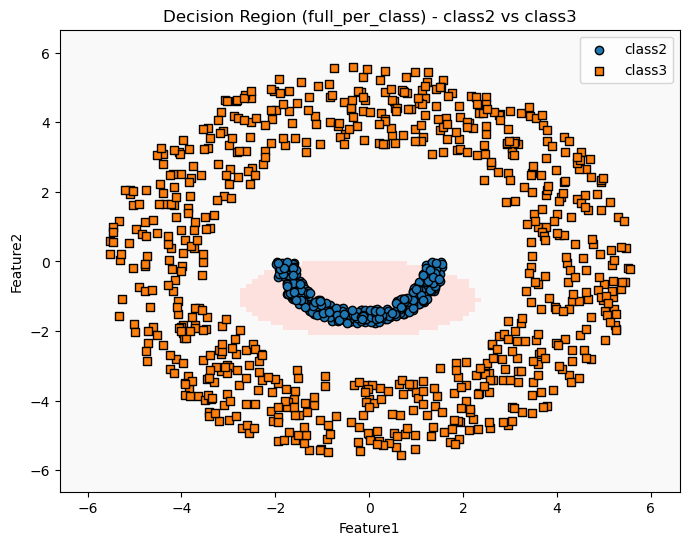
\includegraphics[width=\linewidth]{images/NLS_Group04_images/04_full_per_class/04_decision_region_c2_c3.png}
        \caption*{Class 2 vs Class 3}
    \end{minipage}
    \caption{Decision Region Plots (Training data points superimposed) between class pairs for Full Covariance (Per-Class) on NLS dataset}
\end{figure}